\subsection{Das Interface/Die App}
\label{ssec:interface}
	%Beschreibung der App-Funktionen
	%Benutzeroberfläche und Interaktion

	\subsubsection{Realisierung}
	\label{sssec:realisierung}
		%Implementierte Features und Funktionen
		%Herausforderungen bei der Umsetzung
		
		Die App bietet eine Benutzeroberfläche mit verschiedenen Bildschirmen:
		\begin{figure}[h]
			\centering
			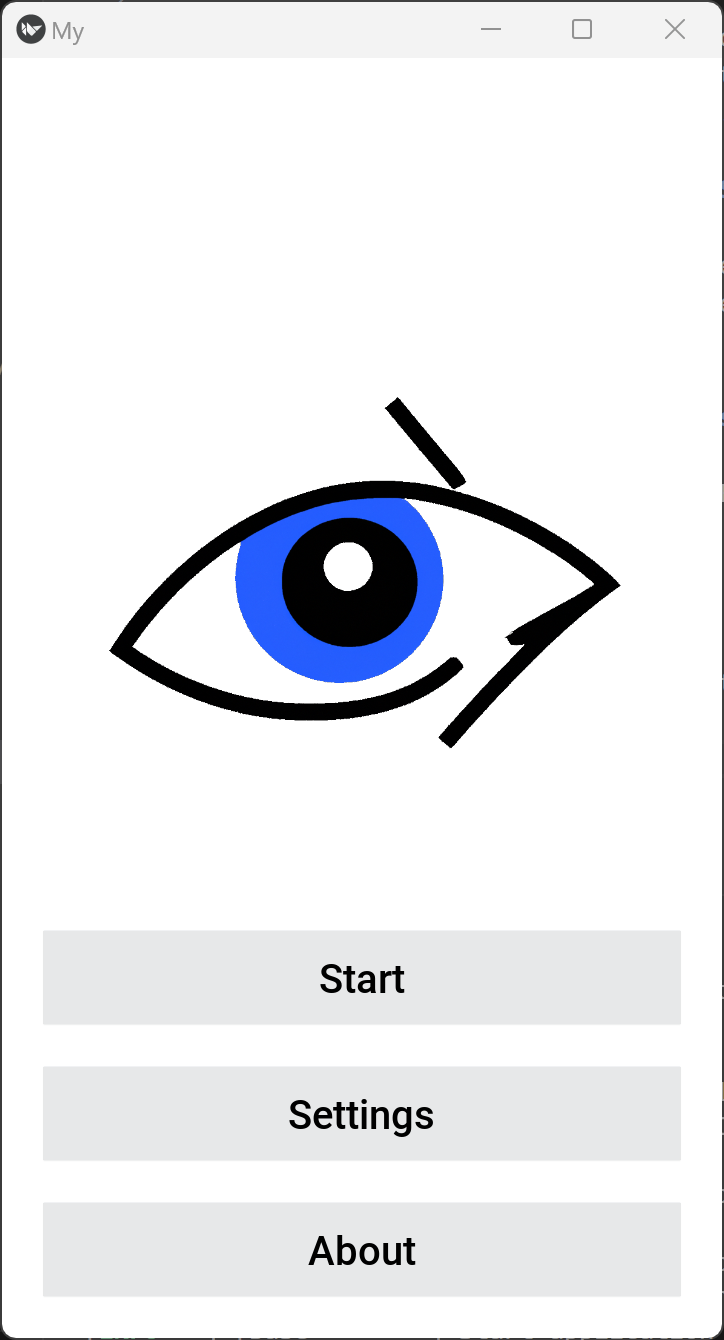
\includegraphics[width=5cm]{images/mainscreen.png} % Ersetzen Sie 'path_to_the_logo.jpg' durch den Pfad zum Logo
			\caption{Hauptbildschirm (MainScreen)}
			\label{fig:mainscreen}
		\end{figure}
		Dies ist der Einstiegsbildschirm der App. Hier erhalten Benutzer eine kurze Einführung in die App und können die Müdigkeitserkennung starten oder auf die Einstellungen zugreifen.
		\begin{figure}[h]
			\centering
			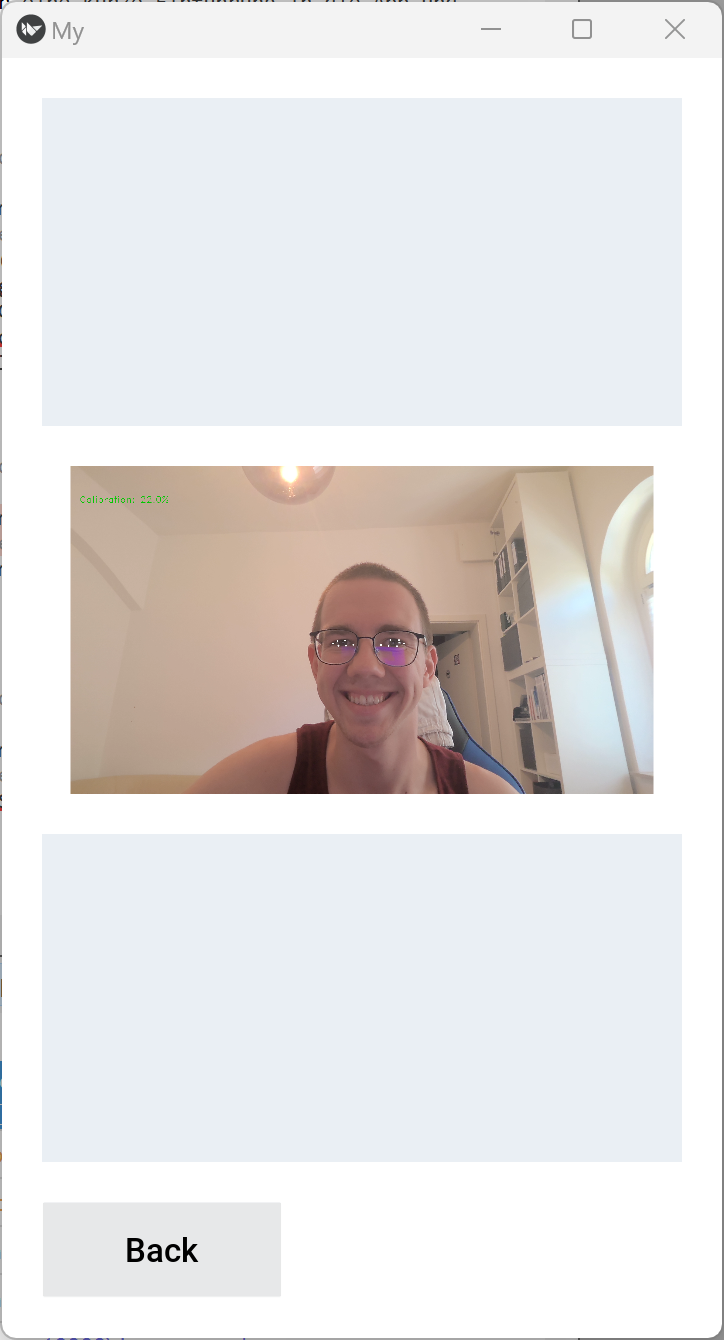
\includegraphics[width=5cm]{images/detectionscreen.png} % Ersetzen Sie 'path_to_the_logo.jpg' durch den Pfad zum Logo
			\caption{Erkennungsbildschirm (DetectionScreen)}
			\label{fig:detectionscreen}
		\end{figure}
		Hier findet die eigentliche Müdigkeitserkennung statt. Die Kamera zeigt eine Echtzeitansicht, und erkannte Gesichtsmerkmale wie die Augen werden markiert. Bei Erkennung von Müdigkeitsmerkmalen kann die App Warnungen anzeigen oder Alarmtöne abspielen.
		\begin{figure}[h]
			\centering
			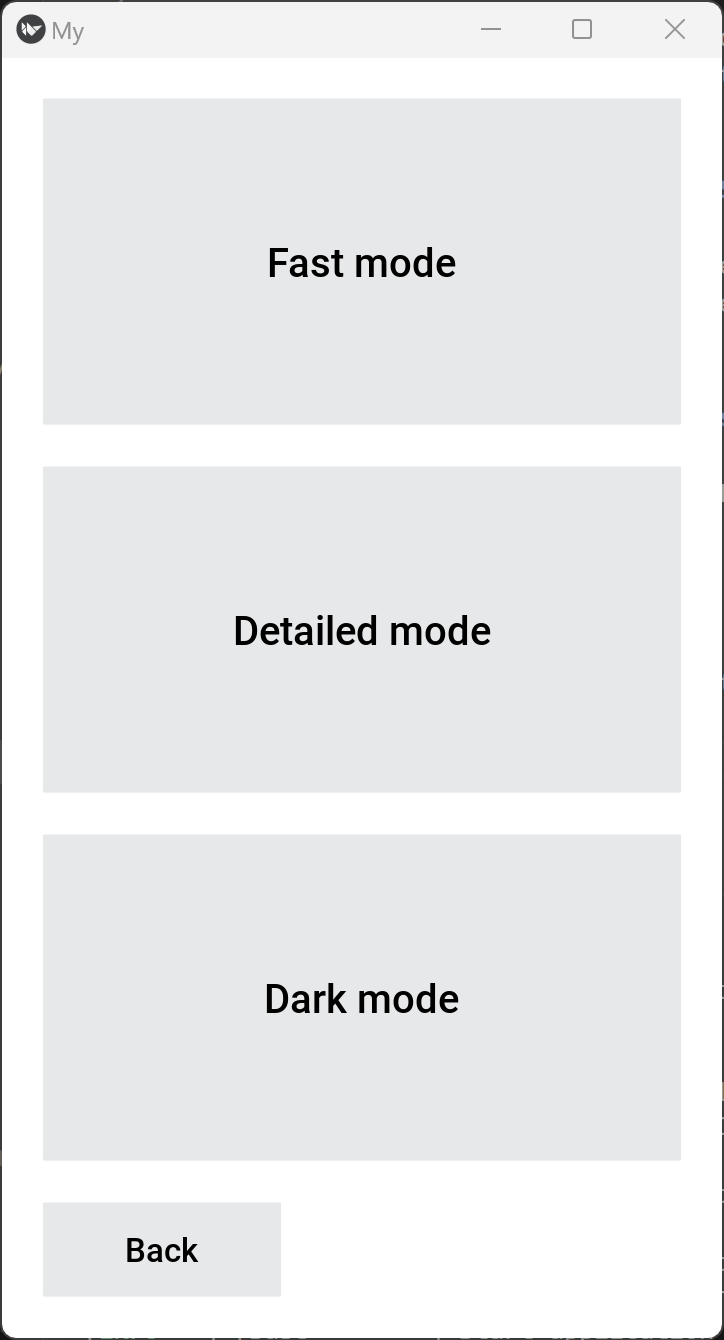
\includegraphics[width=5cm]{images/settingscreen.png} % Ersetzen Sie 'path_to_the_logo.jpg' durch den Pfad zum Logo
			\caption{Einstellungsbildschirm (SettingsScreen)}
			\label{fig:settingscreen}
		\end{figure}
		Benutzer können hier verschiedene Einstellungen für die Benutzeröberfläche anpassen.
		\begin{figure}[h]
			\centering
			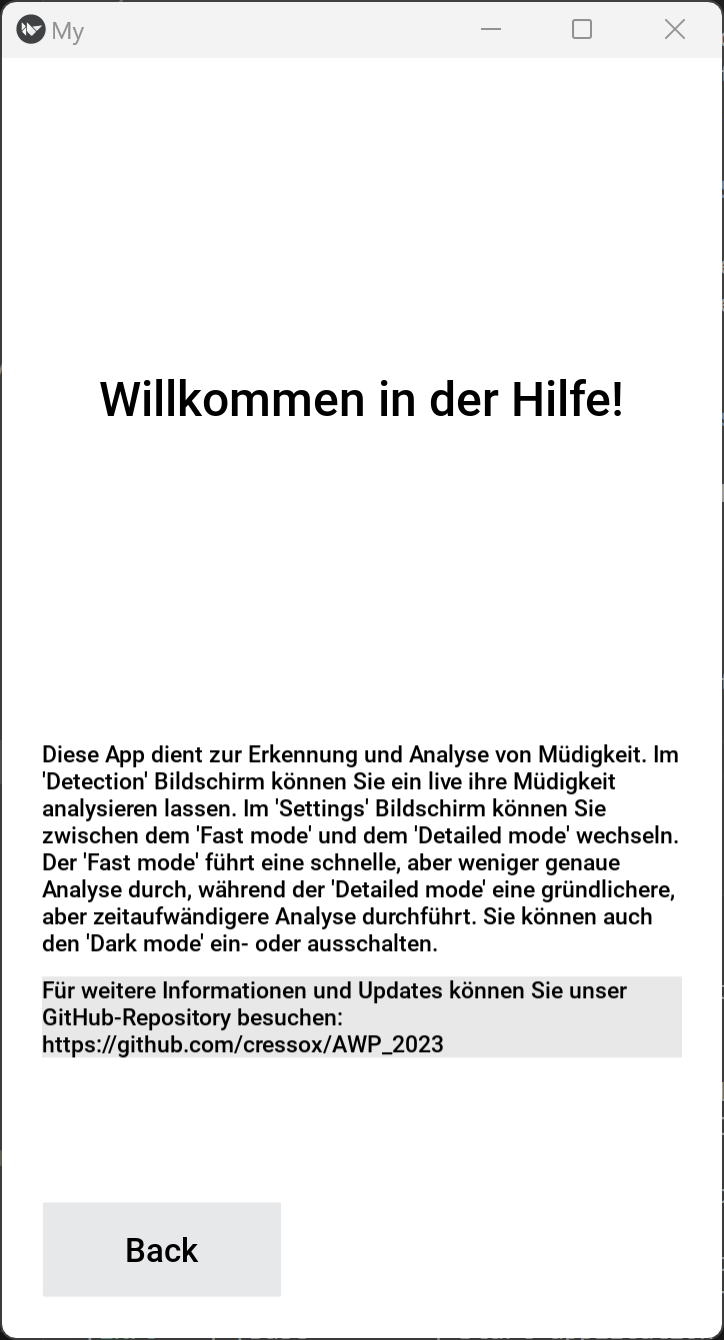
\includegraphics[width=5cm]{images/helpscreen.png} % Ersetzen Sie 'path_to_the_logo.jpg' durch den Pfad zum Logo
			\caption{Hilfebildschirm (HelpScreen)}
			\label{fig:helpscreen}
		\end{figure}
		Dieser Bildschirm bietet detaillierte Informationen zur Verwendung der App und ihrer Funktionen.